% 1980 年全国卷（文科）第 7 题：长方体 ABCD-A'B'C'D'（AB=6、AD=8、AA'=3.6），底面对角线 B'D' 及 AE、A'E（E 为垂足）；左上、显示 A-A' 等被遮棱为虚线（按源卷布局）
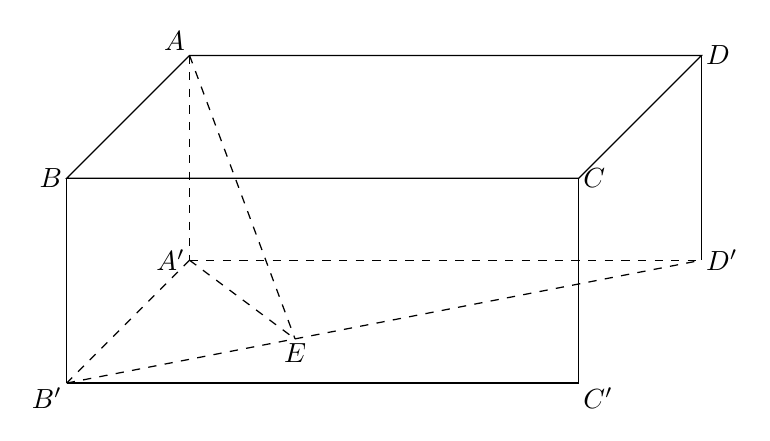
\begin{tikzpicture}[scale=1, line width=0.45pt,
  every node/.style={inner sep=1.5pt}]
  % 顶点（斜二测投影手算：宽 8 单位 -> 6.5cm 水平；深 6 单位 -> 2.2cm 左下 45 度；
  % 高 3.6 单位 -> 2.6cm 竖直）
  \coordinate (A)  at (2.40, 5.80);
  \coordinate (B)  at (0.84, 4.24);
  \coordinate (C)  at (7.34, 4.24);
  \coordinate (D)  at (8.90, 5.80);
  \coordinate (Ap) at (2.40, 3.20);
  \coordinate (Bp) at (0.84, 1.64);
  \coordinate (Cp) at (7.34, 1.64);
  \coordinate (Dp) at (8.90, 3.20);
  % E 为 B'D' 上一点，B'E:B'D' = 3.6:10
  \coordinate (E)  at (3.74, 2.20);
  % 可见棱
  \draw (A) -- (B) -- (C) -- (D) -- cycle;
  \draw (B) -- (Bp);
  \draw (C) -- (Cp);
  \draw (D) -- (Dp);
  \draw (Bp) -- (Cp);
  % 不可见棱（虚线）
  \draw[dashed] (A) -- (Ap);
  \draw[dashed] (Ap) -- (Bp);
  \draw[dashed] (Ap) -- (Dp);
  \draw[dashed] (Bp) -- (Dp);
  \draw[dashed] (A) -- (E);
  \draw[dashed] (Ap) -- (E);
  % 顶点标注
  \node[anchor=south east] at (A)  {$A$};
  \node[anchor=east]       at (B)  {$B$};
  \node[anchor=west]       at (C)  {$C$};
  \node[anchor=west]       at (D)  {$D$};
  \node[anchor=east]       at (Ap) {$A'$};
  \node[anchor=north east] at (Bp) {$B'$};
  \node[anchor=north west] at (Cp) {$C'$};
  \node[anchor=west]       at (Dp) {$D'$};
  \node[anchor=north]      at (E)  {$E$};
\end{tikzpicture}
